\documentclass[11pt]{article}

\author{Computing Workshop}
\title{Simulating a Neural Network}
\date{Fall 2018}

\usepackage[margin=2.0cm]{geometry}
\usepackage{listings}
\usepackage{amsmath}
\usepackage{tikz}
\usetikzlibrary{arrows}

\lstset{
  basicstyle=\ttfamily
}

\begin{document}

\maketitle

In this activity, you will simulate how a neural network classifies an input
point, and how a neural network is trained. You will be working with the iris
dataset. Recall that this dataset is $4$-dimensional, meaning that each data
point has four measurements associated with it. Each data point is assigned one
of three labels, which represents which species of flower those measurements
correspond to.

\section{Getting started}

The idea is that each person in your team will be representing one or more
neurons in the network.

\begin{enumerate}
\item
  Each member of your team opens \emph{the same} Jupyter notebook.
  This way, you can all share data.

  Since the notebook state is shared by all users,
  \textbf{be very careful about evaluating cells in the notebook}.
  Evaluating the wrong cell at the wrong time could mess up someone else's
  data!

\item
  Decide which members of your team are responsible for controlling which
  neurons in the network. Specifically, notice the definitions of the neurons
  \lstinline!p1!, \lstinline!p2!, \lstinline!o1!, \lstinline!o2!, and
  \lstinline!o3!. Each neuron must be assigned so someone in your team.

\item
  Decide on a team leader. The leader will be responsible for setting the inputs
  to the network and reading the outputs of the network.
\end{enumerate}

Fill in the roles you decided on in this table.

\begin{center}
  \begin{tabular}{| c | p{15em} |}
    \hline
    \textbf{$p_1$} & ~ \\ \hline
    \textbf{$p_2$} & ~ \\ \hline
    \textbf{$o_1$} & ~ \\ \hline
    \textbf{$o_2$} & ~ \\ \hline
    \textbf{$o_3$} & ~ \\ \hline
    \textbf{leader} & ~ \\ \hline
  \end{tabular}
\end{center}

For reference, the network you are simulating looks like this.
\begin{center}
  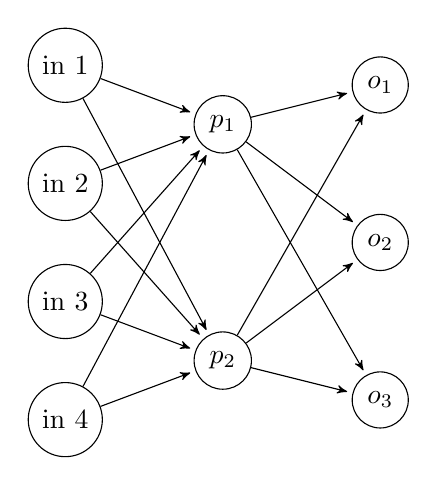
\begin{tikzpicture}[->, >=stealth', shorten >=2pt]
    \node[draw, circle] at (-4, 2.25) (n 1 1)  {in 1};
    \node[draw, circle] at (-4, 0.75) (n 1 2)  {in 2};
    \node[draw, circle] at (-4, -0.75) (n 1 3) {in 3};
    \node[draw, circle] at (-4, -2.25) (n 1 4) {in 4};

    \node[draw, circle] at (-2, 1.5) (n 2 1) {$p_1$};
    \node[draw, circle] at (-2, -1.5) (n 2 2) {$p_2$};

    \node[draw, circle] at (0, 2) (n 3 1) {$o_1$};
    \node[draw, circle] at (0, 0) (n 3 2) {$o_2$};
    \node[draw, circle] at (0, -2) (n 3 3) {$o_3$};

    \foreach \x in {1,2,3,4}
    \foreach \y in {1,2}
    \draw (n 1 \x) -- (n 2 \y);

    \foreach \x in {1,2}
    \foreach \y in {1,2,3}
    \draw (n 2 \x) -- (n 3 \y);

  \end{tikzpicture}
\end{center}

\begin{description}
\item[Leader:]
  run the two cells in the section labelled ``Simulating a neural
  network''. This will load the neural network learner code and prepare the
  iris dataset for you to use.
\item[Leader:]
  run the cells in the section labelled ``Preparing the network.''
\item[Each neuron:]
  run \emph{your cell} in the section ``Check the initial weights''.
\end{description}

To confirm, the weights for neuron $o_1$ should be $[0.3968, 0.9106]$.

Then, follow the sequence of cells in the notebook very carefully, and you
should simulate the function and training of a neural network!

When you get to the section labelled ``Stochastic gradient descent'', let one of
us know!

% \section{Computing feedforward}
% 
% To compute a feedforward through the network, follow these steps.
% \begin{enumerate}
% \item
%   The leader sets the input to the network.
% 
%   Leader: look for the cell labelled ``setting the input''
% \end{enumerate}
% 
% \section{Multilayer perceptron theory}
% 
% To classify an input point, the network needs to perform a \emph{feedforward}.
% 
% Before moving on to how feedforward works in a multilayer perceptron, let's
% recall how it works in a single perceptron. Consider the following perceptron.
% 
% \begin{figure}[h]
%   \centering
%   \begin{tikzpicture}[->, >=stealth', shorten >=1pt, semithick]
%     \node at (-2, 1.75) (input1) {$a^1_1$};
%     \node at (-2, 0) (input2) {$a^1_2$};
%     \node at (-2, -1.75) (input3) {$a^1_3$};
%     \node[draw, circle] at (0, 0) (neuron) {$b^2_1$};
%     \node at (2, 0) (output) {$a^2_1$};
% 
%     \draw (input1) to[edge node={node [above] {$w^2_1$}}] (neuron);
%     \draw (input2) to[edge node={node [above] {$w^2_2$}}] (neuron);
%     \draw (input3) to[edge node={node [above] {$w^2_3$}}] (neuron);
% 
%     \draw (neuron) -- (output);
%   \end{tikzpicture}
% \end{figure}
% 
% It has three inputs $a^1_1$, $a^1_2$, and $a^1_3$ and one output $a^2_1$. The
% inputs and outputs of neurons are called \emph{activations}.
% The superscripts do not denote exponents! There're also indices, denoting which
% \emph{layer} the activation is coming from. We start thinking about layers right
% away in this single perceptron to make the generalization to multilayer
% perceptrons less of a jump. In this example, layer $1$ is the input layer and
% layer $2$ is the output layer, consisting of a single neuron.
% 
% To compute its output $a^2_1$, the neuron first calculates an intermediate
% quantity $z^2_1$ called its \emph{weighted input sum} by multiplying each
% activation from the previous layer by its respective weight and by adding the
% bias $b^2_1$. We can write this as an
% equation.
% \begin{equation*}
%   z^2_1 = w^2_1 a^1_1 + w^2_2 a^1_2 + w^2_3 a^1_3 + b^2_1
% \end{equation*}
% And this equation can be rewritten more compactly using this notation.
% \begin{equation*}
%   z^2_1 = b^2_1 + \sum_{j=1}^3 w^2_j a^1_j
% \end{equation*}
% 
% \emph{In general:} $z^l_j$ denotes the \emph{weighted input sum} of neuron $j$
% in layer $l$ and can be computed using the above expression.
% 
% % exercise about translating this into code?
% 
% In the case of the single perceptron, the output is a binary value $0$ or $1$
% determined by comparing $z^2_1$ against a \emph{threshold} -- e.g. if $z^2_1 > 0$,
% then the output of the neuron is $1$; otherwise, the output is $0$.
% But in a multilayer perceptron, the output is computed by feeding $z^2_1$ into
% some nonlinear function called the \emph{activation function}. A common choice
% for the activation function is the \emph{sigmoid function}, written $\sigma(x)$
% which is defined by
% \begin{equation*}
%   \sigma(x) = \frac{1}{1 + e^{-x}}
% \end{equation*}
% 
% To see how this works, you will compute a feedforward by hand.
% This follows the same idea as for a single perceptron: the activation of a
% neuron is a weighted sum of its inputs, plus a bias. There is one additional
% quirk in the multilayer perceptron: this weighted input sum is passed through a
% \emph{nonlinear} function. In the notebook, this is the function
% \lstinline!sigmoid!.
% 
% \emph{Notation:} we write $a^l_j$ for the activation of neuron $j$ in layer
% $l$. This activation will be defined in terms of the \emph{weighted input sum}
% of neuron $j$ in layer $l$, which we write $z^l_j$.
% 
% The equation for the \emph{weighted input sum} of neuron $j$ in layer $l$ is
% \begin{equation*}
%   z^l_j = b_j^l + \sum_k w^l_{jk} a_k^{l-1}
% \end{equation*}
% where $w^l_{jk}$ is the weight of the connection between neuron $j$ in layer $l$
% neuron $k$ in the layer $l-1$.
% 
% The \emph{activation} of neuron $j$ in layer $l$ is then given by
% \begin{equation*}
%   a^l_j = \sigma(z^l_j)
% \end{equation*}
% 
% For example, consider the network
% %todo diagram
% 
% As you can see, this is a tedious process, so we automated it in the notebook
% for you. Each neuron has the function \lstinline!activate! which computes its
% activation. You can call it by writing \lstinline!p1.activate()! for example.



\end{document}
